\documentclass[../practica_04.tex]{subfiles}

\begin{document}

    $ f(x,y) = \left\{
    \begin{array}{ll}
        \frac{x^3y-xy^3}{x^2+y^2} \quad si\ (x,y)\neq(0,0)\\
        0 \quad si\ (x,y)=(0,0)\\
    \end{array}
    \right.$

    \begin{enumerate}
        \item 
            $ 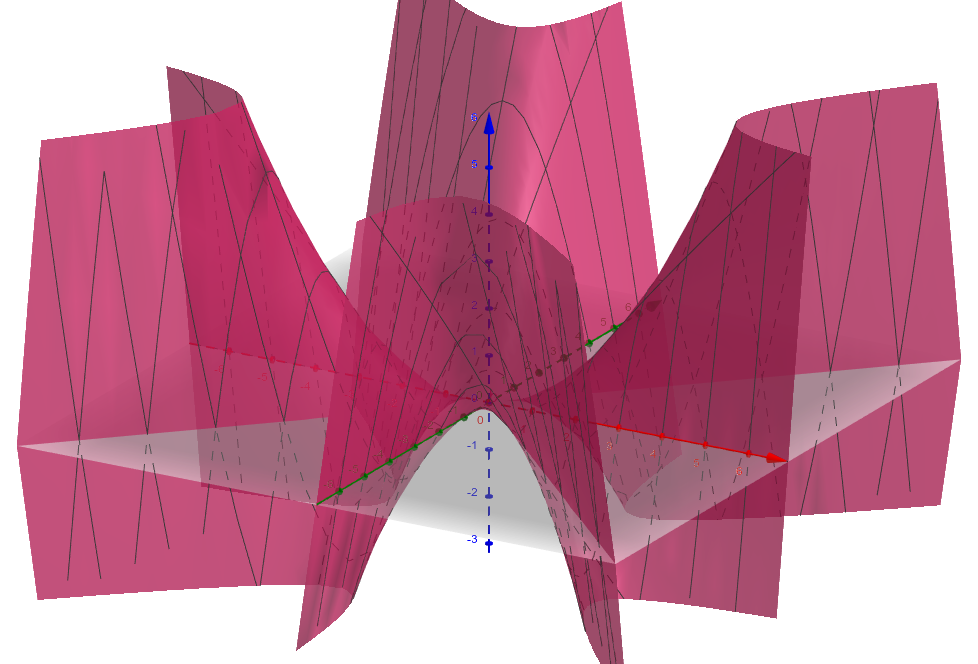
\includegraphics[scale=0.3]{ej08/resources/8a.png} $ 

        \item 
        
            \begin{itemize}
                \item $f_x(x,y) = \frac{y(x^4+4x^2y^2-y^4)}{(x^2+y^2)^2} $
                \item $f_y(x,y) = \frac{x^5-4x^3y^2-xy^4}{(x^2+y^2)^2}$
            \end{itemize}

        \item 

            \begin{itemize}
                \item $f_x(0,0) = \lim_{h\to0} \frac{0}{h^2} = 0 $
                \item $f_y(0,0) = \lim_{h\to0} \frac{0}{h^2} = 0 $
            \end{itemize}

        \item 

            \begin{itemize}
                \item $f_xy(0,0) = \lim_{h\to0} \frac{-y^5)}{y^4} = -1$
                \item $f_yx(0,0) = \lim_{h\to0} \frac{x^5}{x^4} = 1$
            \end{itemize}

        \item No se contradice porque no son continuas

    \end{enumerate}

\end{document}
